\documentclass[twoside]{book}

% Packages required by doxygen
\usepackage{fixltx2e}
\usepackage{calc}
\usepackage{doxygen}
\usepackage[export]{adjustbox} % also loads graphicx
\usepackage{graphicx}
\usepackage[utf8]{inputenc}
\usepackage{makeidx}
\usepackage{multicol}
\usepackage{multirow}
\PassOptionsToPackage{warn}{textcomp}
\usepackage{textcomp}
\usepackage[nointegrals]{wasysym}
\usepackage[table]{xcolor}

% Font selection
\usepackage[T1]{fontenc}
\usepackage[scaled=.90]{helvet}
\usepackage{courier}
\usepackage{amssymb}
\usepackage{sectsty}
\renewcommand{\familydefault}{\sfdefault}
\allsectionsfont{%
  \fontseries{bc}\selectfont%
  \color{darkgray}%
}
\renewcommand{\DoxyLabelFont}{%
  \fontseries{bc}\selectfont%
  \color{darkgray}%
}
\newcommand{\+}{\discretionary{\mbox{\scriptsize$\hookleftarrow$}}{}{}}

% Page & text layout
\usepackage{geometry}
\geometry{%
  a4paper,%
  top=2.5cm,%
  bottom=2.5cm,%
  left=2.5cm,%
  right=2.5cm%
}
\tolerance=750
\hfuzz=15pt
\hbadness=750
\setlength{\emergencystretch}{15pt}
\setlength{\parindent}{0cm}
\setlength{\parskip}{3ex plus 2ex minus 2ex}
\makeatletter
\renewcommand{\paragraph}{%
  \@startsection{paragraph}{4}{0ex}{-1.0ex}{1.0ex}{%
    \normalfont\normalsize\bfseries\SS@parafont%
  }%
}
\renewcommand{\subparagraph}{%
  \@startsection{subparagraph}{5}{0ex}{-1.0ex}{1.0ex}{%
    \normalfont\normalsize\bfseries\SS@subparafont%
  }%
}
\makeatother

% Headers & footers
\usepackage{fancyhdr}
\pagestyle{fancyplain}
\fancyhead[LE]{\fancyplain{}{\bfseries\thepage}}
\fancyhead[CE]{\fancyplain{}{}}
\fancyhead[RE]{\fancyplain{}{\bfseries\leftmark}}
\fancyhead[LO]{\fancyplain{}{\bfseries\rightmark}}
\fancyhead[CO]{\fancyplain{}{}}
\fancyhead[RO]{\fancyplain{}{\bfseries\thepage}}
\fancyfoot[LE]{\fancyplain{}{}}
\fancyfoot[CE]{\fancyplain{}{}}
\fancyfoot[RE]{\fancyplain{}{\bfseries\scriptsize Generated by Doxygen }}
\fancyfoot[LO]{\fancyplain{}{\bfseries\scriptsize Generated by Doxygen }}
\fancyfoot[CO]{\fancyplain{}{}}
\fancyfoot[RO]{\fancyplain{}{}}
\renewcommand{\footrulewidth}{0.4pt}
\renewcommand{\chaptermark}[1]{%
  \markboth{#1}{}%
}
\renewcommand{\sectionmark}[1]{%
  \markright{\thesection\ #1}%
}

% Indices & bibliography
\usepackage{natbib}
\usepackage[titles]{tocloft}
\setcounter{tocdepth}{3}
\setcounter{secnumdepth}{5}
\makeindex

% Hyperlinks (required, but should be loaded last)
\usepackage{ifpdf}
\ifpdf
  \usepackage[pdftex,pagebackref=true]{hyperref}
\else
  \usepackage[ps2pdf,pagebackref=true]{hyperref}
\fi
\hypersetup{%
  colorlinks=true,%
  linkcolor=blue,%
  citecolor=blue,%
  unicode%
}

% Custom commands
\newcommand{\clearemptydoublepage}{%
  \newpage{\pagestyle{empty}\cleardoublepage}%
}

\usepackage{caption}
\captionsetup{labelsep=space,justification=centering,font={bf},singlelinecheck=off,skip=4pt,position=top}

%===== C O N T E N T S =====

\begin{document}

% Titlepage & ToC
\hypersetup{pageanchor=false,
             bookmarksnumbered=true,
             pdfencoding=unicode
            }
\pagenumbering{roman}
\begin{titlepage}
\vspace*{7cm}
\begin{center}%
{\Large HW 5 -\/ Matrix Class }\\
\vspace*{1cm}
{\large Generated by Doxygen 1.8.11}\\
\end{center}
\end{titlepage}
\clearemptydoublepage
\tableofcontents
\clearemptydoublepage
\pagenumbering{arabic}
\hypersetup{pageanchor=true}

%--- Begin generated contents ---
\chapter{C\+S5201\+\_\+\+H\+W5}
\label{md_README}
\hypertarget{md_README}{}
\section*{C\+S5201\+\_\+\+H\+W5}
\chapter{Class Index}
\section{Class List}
Here are the classes, structs, unions and interfaces with brief descriptions\+:\begin{DoxyCompactList}
\item\contentsline{section}{\hyperlink{classCompare}{Compare$<$ T $>$} }{\pageref{classCompare}}{}
\item\contentsline{section}{\hyperlink{classGauss}{Gauss$<$ T $>$} }{\pageref{classGauss}}{}
\item\contentsline{section}{\hyperlink{classMatrix}{Matrix$<$ T $>$} }{\pageref{classMatrix}}{}
\item\contentsline{section}{\hyperlink{classMyArray}{My\+Array$<$ T $>$} }{\pageref{classMyArray}}{}
\end{DoxyCompactList}

\chapter{File Index}
\section{File List}
Here is a list of all documented files with brief descriptions\+:\begin{DoxyCompactList}
\item\contentsline{section}{\hyperlink{Gauss_8h}{Gauss.\+h} }{\pageref{Gauss_8h}}{}
\item\contentsline{section}{{\bfseries Gauss.\+hpp} }{\pageref{Gauss_8hpp}}{}
\item\contentsline{section}{\hyperlink{matrix_8h}{matrix.\+h} }{\pageref{matrix_8h}}{}
\item\contentsline{section}{{\bfseries matrix.\+hpp} }{\pageref{matrix_8hpp}}{}
\item\contentsline{section}{\hyperlink{myArray_8h}{my\+Array.\+h} }{\pageref{myArray_8h}}{}
\item\contentsline{section}{{\bfseries my\+Array.\+hpp} }{\pageref{myArray_8hpp}}{}
\end{DoxyCompactList}

\chapter{Class Documentation}
\hypertarget{classCompare}{}\section{Compare$<$ T $>$ Class Template Reference}
\label{classCompare}\index{Compare$<$ T $>$@{Compare$<$ T $>$}}


{\ttfamily \#include $<$matrix.\+h$>$}

\subsection*{Public Member Functions}
\begin{DoxyCompactItemize}
\item 
bool \hyperlink{classCompare_a6024147b908ca76c18ef56bc59f59147}{operator()} (const tuple$<$ T, int $>$ lhs, const tuple$<$ T, int $>$ rhs) const 
\end{DoxyCompactItemize}


\subsection{Detailed Description}
\subsubsection*{template$<$typename T$>$\\*
class Compare$<$ T $>$}

The compare Class. 

\subsection{Member Function Documentation}
\index{Compare@{Compare}!operator()@{operator()}}
\index{operator()@{operator()}!Compare@{Compare}}
\subsubsection[{\texorpdfstring{operator()(const tuple$<$ T, int $>$ lhs, const tuple$<$ T, int $>$ rhs) const }{operator()(const tuple< T, int > lhs, const tuple< T, int > rhs) const }}]{\setlength{\rightskip}{0pt plus 5cm}template$<$typename T $>$ bool {\bf Compare}$<$ T $>$\+::operator() (
\begin{DoxyParamCaption}
\item[{const tuple$<$ T, int $>$}]{lhs, }
\item[{const tuple$<$ T, int $>$}]{rhs}
\end{DoxyParamCaption}
) const\hspace{0.3cm}{\ttfamily [inline]}}\hypertarget{classCompare_a6024147b908ca76c18ef56bc59f59147}{}\label{classCompare_a6024147b908ca76c18ef56bc59f59147}
The () Operator returns true if lhs $<$ rhs \begin{DoxyPrecond}{Precondition}
\textquotesingle{}$<$\textquotesingle{} operator defind for T! 
\end{DoxyPrecond}
\begin{DoxyPostcond}{Postcondition}
none 
\end{DoxyPostcond}


The documentation for this class was generated from the following file\+:\begin{DoxyCompactItemize}
\item 
\hyperlink{matrix_8h}{matrix.\+h}\end{DoxyCompactItemize}

\hypertarget{classGauss}{}\section{Gauss$<$ T $>$ Class Template Reference}
\label{classGauss}\index{Gauss$<$ T $>$@{Gauss$<$ T $>$}}


{\ttfamily \#include $<$Gauss.\+h$>$}

\subsection*{Public Member Functions}
\begin{DoxyCompactItemize}
\item 
\hyperlink{classMyArray}{My\+Array}$<$ T $>$ \hyperlink{classGauss_a26c6cb82642023d213f05723f23af627}{operator()} (const \hyperlink{classMatrix}{Matrix}$<$ T $>$ \&mat, const \hyperlink{classMyArray}{My\+Array}$<$ T $>$ \&vec) const 
\end{DoxyCompactItemize}


\subsection{Detailed Description}
\subsubsection*{template$<$typename T$>$\\*
class Gauss$<$ T $>$}

the \hyperlink{classGauss}{Gauss} solver calculation class 

\subsection{Member Function Documentation}
\index{Gauss@{Gauss}!operator()@{operator()}}
\index{operator()@{operator()}!Gauss@{Gauss}}
\subsubsection[{\texorpdfstring{operator()(const Matrix$<$ T $>$ \&mat, const My\+Array$<$ T $>$ \&vec) const }{operator()(const Matrix< T > &mat, const MyArray< T > &vec) const }}]{\setlength{\rightskip}{0pt plus 5cm}template$<$typename T $>$ {\bf My\+Array}$<$ T $>$ {\bf Gauss}$<$ T $>$\+::operator() (
\begin{DoxyParamCaption}
\item[{const {\bf Matrix}$<$ T $>$ \&}]{mat, }
\item[{const {\bf My\+Array}$<$ T $>$ \&}]{vec}
\end{DoxyParamCaption}
) const}\hypertarget{classGauss_a26c6cb82642023d213f05723f23af627}{}\label{classGauss_a26c6cb82642023d213f05723f23af627}
Operator () calculator! \textbackslash{} Calcultes the \hyperlink{classGauss}{Gauss} algorthem for the Ax=b eqation. A is the mat \hyperlink{classMatrix}{Matrix}. b Is the vec \hyperlink{classMyArray}{My\+Array}. \begin{DoxyPrecond}{Precondition}
\char`\"{}-\/\char`\"{} binary operator defiend for T pre \char`\"{}$\ast$\char`\"{} binary operator defiend for T 
\end{DoxyPrecond}
\begin{DoxyPostcond}{Postcondition}
A new \hyperlink{classMyArray}{My\+Array} is born 
\end{DoxyPostcond}
\begin{DoxyReturn}{Returns}
a new Array with the calculated results. 
\end{DoxyReturn}


The documentation for this class was generated from the following files\+:\begin{DoxyCompactItemize}
\item 
\hyperlink{Gauss_8h}{Gauss.\+h}\item 
Gauss.\+hpp\end{DoxyCompactItemize}

\hypertarget{classMatrix}{}\section{Matrix$<$ T $>$ Class Template Reference}
\label{classMatrix}\index{Matrix$<$ T $>$@{Matrix$<$ T $>$}}


{\ttfamily \#include $<$matrix.\+h$>$}

\subsection*{Public Member Functions}
\begin{DoxyCompactItemize}
\item 
\hyperlink{classMatrix_a9d567e3a121b1be0c3f9c461cab524fe}{Matrix} ()
\item 
\hyperlink{classMatrix_a19ffa179320a60ab6aeb0910f062895f}{Matrix} (const int n)
\item 
\hyperlink{classMatrix_a6a46705243036bfeee78fe2c84c54340}{Matrix} (const \hyperlink{classMatrix}{Matrix}$<$ T $>$ \&rhs)
\item 
\hyperlink{classMatrix_a91aa704de674203e96aece9e1955ccd3}{$\sim$\+Matrix} ()
\item 
\hyperlink{classMatrix}{Matrix}$<$ T $>$ \& \hyperlink{classMatrix_a01990eb2552555d37c83272125be68e6}{operator=} (const \hyperlink{classMatrix}{Matrix}$<$ T $>$ \&rhs)
\item 
\hyperlink{classMatrix_ac503fc6ce19453907fd9ad85133fef39}{Matrix} (\hyperlink{classMatrix}{Matrix} \&\&rhs)
\item 
\hyperlink{classMatrix}{Matrix}$<$ T $>$ \hyperlink{classMatrix_a9db4b4074daa2112eab910c7902fc5d9}{operator+} (const \hyperlink{classMatrix}{Matrix}$<$ T $>$ \&rhs) const 
\item 
\hyperlink{classMatrix}{Matrix}$<$ T $>$ \hyperlink{classMatrix_a06a7f018ed353f0a8239a80ec8403be6}{operator-\/} (const \hyperlink{classMatrix}{Matrix}$<$ T $>$ \&rhs) const 
\item 
\hyperlink{classMatrix}{Matrix}$<$ T $>$ \hyperlink{classMatrix_a358516deb804403fb91256a5a269d1e2}{operator$\ast$} (const \hyperlink{classMatrix}{Matrix}$<$ T $>$ \&rhs) const 
\item 
\hyperlink{classMyArray}{My\+Array}$<$ T $>$ \hyperlink{classMatrix_a70c46247336f74291cc3e1b2fb800a34}{operator$\ast$} (const \hyperlink{classMyArray}{My\+Array}$<$ T $>$ \&rhs) const 
\item 
\hyperlink{classMyArray}{My\+Array}$<$ T $>$ \& \hyperlink{classMatrix_a47c3685edce37163855474b360d91202}{operator\mbox{[}$\,$\mbox{]}} (const int i) const 
\item 
void \hyperlink{classMatrix_aba8c673e5ca3bcc56a9bad1a1c0fed23}{scaler\+Multi} (const T scaler)
\item 
void \hyperlink{classMatrix_a23bb949d4b4256dd253808e35d73d4b9}{switch\+Rows} (const int i, const int j)
\item 
int \hyperlink{classMatrix_aa5d12d49bec4b4876f1a60c54a197ed7}{get\+Size} () const 
\item 
void \hyperlink{classMatrix_ad7a4ff9efa74bf23786446262bffd043}{set\+Size} (int s)
\item 
\hyperlink{classMatrix}{Matrix}$<$ T $>$ \hyperlink{classMatrix_afe686234b6fe54ab2ae7f500777ca560}{transpose} () const 
\end{DoxyCompactItemize}
\subsection*{Friends}
\begin{DoxyCompactItemize}
\item 
ostream \& \hyperlink{classMatrix_a7a26ce88f9d928002eba0af6847a0b44}{operator} (ostream \&out, \hyperlink{classMatrix}{Matrix}$<$ T $>$ \&mat)
\end{DoxyCompactItemize}


\subsection{Detailed Description}
\subsubsection*{template$<$class T$>$\\*
class Matrix$<$ T $>$}

\hyperlink{classMatrix}{Matrix} calss Reprents a NxN \hyperlink{classMatrix}{Matrix} contains a\+: m\+\_\+size -\/ represting the size of N m\+\_\+matrix -\/ an my\+Array of my\+Arrays represting the matrix 

\subsection{Constructor \& Destructor Documentation}
\index{Matrix@{Matrix}!Matrix@{Matrix}}
\index{Matrix@{Matrix}!Matrix@{Matrix}}
\subsubsection[{\texorpdfstring{Matrix()}{Matrix()}}]{\setlength{\rightskip}{0pt plus 5cm}template$<$typename T $>$ {\bf Matrix}$<$ T $>$\+::{\bf Matrix} (
\begin{DoxyParamCaption}
{}
\end{DoxyParamCaption}
)}\hypertarget{classMatrix_a9d567e3a121b1be0c3f9c461cab524fe}{}\label{classMatrix_a9d567e3a121b1be0c3f9c461cab524fe}
defult constructor. A new \hyperlink{classMatrix}{Matrix} is craeted with N equals 0. \begin{DoxyPrecond}{Precondition}
none 
\end{DoxyPrecond}
\begin{DoxyPostcond}{Postcondition}
a \hyperlink{classMatrix}{Matrix} is born! 
\end{DoxyPostcond}
\index{Matrix@{Matrix}!Matrix@{Matrix}}
\index{Matrix@{Matrix}!Matrix@{Matrix}}
\subsubsection[{\texorpdfstring{Matrix(const int n)}{Matrix(const int n)}}]{\setlength{\rightskip}{0pt plus 5cm}template$<$typename T $>$ {\bf Matrix}$<$ T $>$\+::{\bf Matrix} (
\begin{DoxyParamCaption}
\item[{const int}]{n}
\end{DoxyParamCaption}
)}\hypertarget{classMatrix_a19ffa179320a60ab6aeb0910f062895f}{}\label{classMatrix_a19ffa179320a60ab6aeb0910f062895f}
initialize constructor. A new \hyperlink{classMatrix}{Matrix} is craeted with dimensions equel to \char`\"{}n\char`\"{} \begin{DoxyPrecond}{Precondition}
size must be bigger then 0! Will throw a a length Error otherwise 
\end{DoxyPrecond}
\begin{DoxyPostcond}{Postcondition}
a \hyperlink{classMatrix}{Matrix} is born! 
\end{DoxyPostcond}
\index{Matrix@{Matrix}!Matrix@{Matrix}}
\index{Matrix@{Matrix}!Matrix@{Matrix}}
\subsubsection[{\texorpdfstring{Matrix(const Matrix$<$ T $>$ \&rhs)}{Matrix(const Matrix< T > &rhs)}}]{\setlength{\rightskip}{0pt plus 5cm}template$<$typename T $>$ {\bf Matrix}$<$ T $>$\+::{\bf Matrix} (
\begin{DoxyParamCaption}
\item[{const {\bf Matrix}$<$ T $>$ \&}]{rhs}
\end{DoxyParamCaption}
)}\hypertarget{classMatrix_a6a46705243036bfeee78fe2c84c54340}{}\label{classMatrix_a6a46705243036bfeee78fe2c84c54340}
copy constructor. A new Marix is craeted with size equel to R\+HS size. \begin{DoxyPrecond}{Precondition}
none 
\end{DoxyPrecond}
\begin{DoxyPostcond}{Postcondition}
a \hyperlink{classMatrix}{Matrix} is born! 
\end{DoxyPostcond}
\index{Matrix@{Matrix}!````~Matrix@{$\sim$\+Matrix}}
\index{````~Matrix@{$\sim$\+Matrix}!Matrix@{Matrix}}
\subsubsection[{\texorpdfstring{$\sim$\+Matrix()}{~Matrix()}}]{\setlength{\rightskip}{0pt plus 5cm}template$<$typename T $>$ {\bf Matrix}$<$ T $>$\+::$\sim${\bf Matrix} (
\begin{DoxyParamCaption}
{}
\end{DoxyParamCaption}
)}\hypertarget{classMatrix_a91aa704de674203e96aece9e1955ccd3}{}\label{classMatrix_a91aa704de674203e96aece9e1955ccd3}
deconstructor.

An Arnold Schwarzenegger Terminates the pointer to avoid Skynet taking over with their memorey Leacks. \char`\"{} Hasta La Vista , Pointer \char`\"{} \index{Matrix@{Matrix}!Matrix@{Matrix}}
\index{Matrix@{Matrix}!Matrix@{Matrix}}
\subsubsection[{\texorpdfstring{Matrix(\+Matrix \&\&rhs)}{Matrix(Matrix &&rhs)}}]{\setlength{\rightskip}{0pt plus 5cm}template$<$class T$>$ {\bf Matrix}$<$ T $>$\+::{\bf Matrix} (
\begin{DoxyParamCaption}
\item[{{\bf Matrix}$<$ T $>$ \&\&}]{rhs}
\end{DoxyParamCaption}
)\hspace{0.3cm}{\ttfamily [inline]}}\hypertarget{classMatrix_ac503fc6ce19453907fd9ad85133fef39}{}\label{classMatrix_ac503fc6ce19453907fd9ad85133fef39}
move constructor. A new \hyperlink{classMatrix}{Matrix} is craeted with Size equel to R\+HS size \begin{DoxyPrecond}{Precondition}
none 
\end{DoxyPrecond}
\begin{DoxyPostcond}{Postcondition}
a \hyperlink{classMatrix}{Matrix} is born! 
\end{DoxyPostcond}


\subsection{Member Function Documentation}
\index{Matrix@{Matrix}!get\+Size@{get\+Size}}
\index{get\+Size@{get\+Size}!Matrix@{Matrix}}
\subsubsection[{\texorpdfstring{get\+Size() const }{getSize() const }}]{\setlength{\rightskip}{0pt plus 5cm}template$<$class T$>$ int {\bf Matrix}$<$ T $>$\+::get\+Size (
\begin{DoxyParamCaption}
{}
\end{DoxyParamCaption}
) const\hspace{0.3cm}{\ttfamily [inline]}}\hypertarget{classMatrix_aa5d12d49bec4b4876f1a60c54a197ed7}{}\label{classMatrix_aa5d12d49bec4b4876f1a60c54a197ed7}
get size!

\begin{DoxyPrecond}{Precondition}
none 
\end{DoxyPrecond}
\begin{DoxyPostcond}{Postcondition}
none 
\end{DoxyPostcond}
\begin{DoxyReturn}{Returns}
size of Martix 
\end{DoxyReturn}
\index{Matrix@{Matrix}!operator$\ast$@{operator$\ast$}}
\index{operator$\ast$@{operator$\ast$}!Matrix@{Matrix}}
\subsubsection[{\texorpdfstring{operator$\ast$(const Matrix$<$ T $>$ \&rhs) const }{operator*(const Matrix< T > &rhs) const }}]{\setlength{\rightskip}{0pt plus 5cm}template$<$typename T $>$ {\bf Matrix}$<$ T $>$ {\bf Matrix}$<$ T $>$\+::{\bf operator}$\ast$ (
\begin{DoxyParamCaption}
\item[{const {\bf Matrix}$<$ T $>$ \&}]{rhs}
\end{DoxyParamCaption}
) const}\hypertarget{classMatrix_a358516deb804403fb91256a5a269d1e2}{}\label{classMatrix_a358516deb804403fb91256a5a269d1e2}
\hyperlink{classMatrix}{Matrix} multiplication caclualtes the multiplication of 2 matrixs and returens a new matrix with the calculated values \begin{DoxyPrecond}{Precondition}
size of CO must be equel to rhs, Will throw a a length Error otherwise. \char`\"{}$\ast$\char`\"{} binary operator must be defiend for T. 
\end{DoxyPrecond}
\begin{DoxyPostcond}{Postcondition}
a matrix is born! 
\end{DoxyPostcond}
\index{Matrix@{Matrix}!operator$\ast$@{operator$\ast$}}
\index{operator$\ast$@{operator$\ast$}!Matrix@{Matrix}}
\subsubsection[{\texorpdfstring{operator$\ast$(const My\+Array$<$ T $>$ \&rhs) const }{operator*(const MyArray< T > &rhs) const }}]{\setlength{\rightskip}{0pt plus 5cm}template$<$typename T $>$ {\bf My\+Array}$<$ T $>$ {\bf Matrix}$<$ T $>$\+::{\bf operator}$\ast$ (
\begin{DoxyParamCaption}
\item[{const {\bf My\+Array}$<$ T $>$ \&}]{rhs}
\end{DoxyParamCaption}
) const}\hypertarget{classMatrix_a70c46247336f74291cc3e1b2fb800a34}{}\label{classMatrix_a70c46247336f74291cc3e1b2fb800a34}
\hyperlink{classMatrix}{Matrix} -\/ Vector multiplication caclualtes the multiplication of 2 of a \hyperlink{classMatrix}{Matrix} with an Array and returens a new Vector with the calculated values \begin{DoxyPrecond}{Precondition}
size of CO must be equel to rhs array size! Will throw a a length Error otherwise. \char`\"{}$\ast$\char`\"{} binary operator must be defiend for T. 
\end{DoxyPrecond}
\begin{DoxyPostcond}{Postcondition}
a Vector is born! 
\end{DoxyPostcond}
\index{Matrix@{Matrix}!operator+@{operator+}}
\index{operator+@{operator+}!Matrix@{Matrix}}
\subsubsection[{\texorpdfstring{operator+(const Matrix$<$ T $>$ \&rhs) const }{operator+(const Matrix< T > &rhs) const }}]{\setlength{\rightskip}{0pt plus 5cm}template$<$typename T $>$ {\bf Matrix}$<$ T $>$ {\bf Matrix}$<$ T $>$\+::{\bf operator}+ (
\begin{DoxyParamCaption}
\item[{const {\bf Matrix}$<$ T $>$ \&}]{rhs}
\end{DoxyParamCaption}
) const}\hypertarget{classMatrix_a9db4b4074daa2112eab910c7902fc5d9}{}\label{classMatrix_a9db4b4074daa2112eab910c7902fc5d9}

\begin{DoxyItemize}
\item operator adds the sum of CO to rhs, retures a new \hyperlink{classMatrix}{Matrix} with the calculated values \begin{DoxyPrecond}{Precondition}
size of CO must be equel to rhs, Will throw a a length Error otherwise. \char`\"{}+\char`\"{} binary operator must be defiend for T. 
\end{DoxyPrecond}
\begin{DoxyPostcond}{Postcondition}
a matrix is born! 
\end{DoxyPostcond}

\end{DoxyItemize}\index{Matrix@{Matrix}!operator-\/@{operator-\/}}
\index{operator-\/@{operator-\/}!Matrix@{Matrix}}
\subsubsection[{\texorpdfstring{operator-\/(const Matrix$<$ T $>$ \&rhs) const }{operator-(const Matrix< T > &rhs) const }}]{\setlength{\rightskip}{0pt plus 5cm}template$<$typename T $>$ {\bf Matrix}$<$ T $>$ {\bf Matrix}$<$ T $>$\+::{\bf operator}-\/ (
\begin{DoxyParamCaption}
\item[{const {\bf Matrix}$<$ T $>$ \&}]{rhs}
\end{DoxyParamCaption}
) const}\hypertarget{classMatrix_a06a7f018ed353f0a8239a80ec8403be6}{}\label{classMatrix_a06a7f018ed353f0a8239a80ec8403be6}

\begin{DoxyItemize}
\item operator caclualtes the differnce of CO to rhs, retures a new \hyperlink{classMatrix}{Matrix} with the calculated values \begin{DoxyPrecond}{Precondition}
size of CO must be equel to rhs, Will throw a a length Error otherwise. \char`\"{}-\/\char`\"{} binary operator must be defiend for T. 
\end{DoxyPrecond}
\begin{DoxyPostcond}{Postcondition}
a matrix is born! 
\end{DoxyPostcond}

\end{DoxyItemize}\index{Matrix@{Matrix}!operator=@{operator=}}
\index{operator=@{operator=}!Matrix@{Matrix}}
\subsubsection[{\texorpdfstring{operator=(const Matrix$<$ T $>$ \&rhs)}{operator=(const Matrix< T > &rhs)}}]{\setlength{\rightskip}{0pt plus 5cm}template$<$typename T $>$ {\bf Matrix}$<$ T $>$ \& {\bf Matrix}$<$ T $>$\+::{\bf operator}= (
\begin{DoxyParamCaption}
\item[{const {\bf Matrix}$<$ T $>$ \&}]{rhs}
\end{DoxyParamCaption}
)}\hypertarget{classMatrix_a01990eb2552555d37c83272125be68e6}{}\label{classMatrix_a01990eb2552555d37c83272125be68e6}
= assignment turns the CO \hyperlink{classMatrix}{Matrix} into R\+HS matix \begin{DoxyPrecond}{Precondition}
none 
\end{DoxyPrecond}
\begin{DoxyPostcond}{Postcondition}
none 
\end{DoxyPostcond}
\index{Matrix@{Matrix}!operator\mbox{[}$\,$\mbox{]}@{operator[]}}
\index{operator\mbox{[}$\,$\mbox{]}@{operator[]}!Matrix@{Matrix}}
\subsubsection[{\texorpdfstring{operator[](const int i) const }{operator[](const int i) const }}]{\setlength{\rightskip}{0pt plus 5cm}template$<$typename T $>$ {\bf My\+Array}$<$ T $>$ \& {\bf Matrix}$<$ T $>$\+::{\bf operator}\mbox{[}$\,$\mbox{]} (
\begin{DoxyParamCaption}
\item[{const int}]{i}
\end{DoxyParamCaption}
) const}\hypertarget{classMatrix_a47c3685edce37163855474b360d91202}{}\label{classMatrix_a47c3685edce37163855474b360d91202}
object getter \mbox{[}\mbox{]}

\begin{DoxyPrecond}{Precondition}
0 $<$ i $<$ size, will throw a a length Error otherwise 
\end{DoxyPrecond}
\begin{DoxyPostcond}{Postcondition}
none 
\end{DoxyPostcond}
\begin{DoxyReturn}{Returns}
Will return the \hyperlink{classMyArray}{My\+Array} at index i. 
\end{DoxyReturn}
\index{Matrix@{Matrix}!scaler\+Multi@{scaler\+Multi}}
\index{scaler\+Multi@{scaler\+Multi}!Matrix@{Matrix}}
\subsubsection[{\texorpdfstring{scaler\+Multi(const T scaler)}{scalerMulti(const T scaler)}}]{\setlength{\rightskip}{0pt plus 5cm}template$<$typename T $>$ void {\bf Matrix}$<$ T $>$\+::scaler\+Multi (
\begin{DoxyParamCaption}
\item[{const T}]{scaler}
\end{DoxyParamCaption}
)}\hypertarget{classMatrix_aba8c673e5ca3bcc56a9bad1a1c0fed23}{}\label{classMatrix_aba8c673e5ca3bcc56a9bad1a1c0fed23}
\hyperlink{classMatrix}{Matrix} Scaler multiplication caclualtes the multiplication of a matrixs with a scaler and modifies the CO m\+\_\+matrix with calculation \begin{DoxyPrecond}{Precondition}
\char`\"{}$\ast$\char`\"{} binary operator must be defiend for T. 
\end{DoxyPrecond}
\begin{DoxyPostcond}{Postcondition}
none 
\end{DoxyPostcond}
\index{Matrix@{Matrix}!set\+Size@{set\+Size}}
\index{set\+Size@{set\+Size}!Matrix@{Matrix}}
\subsubsection[{\texorpdfstring{set\+Size(int s)}{setSize(int s)}}]{\setlength{\rightskip}{0pt plus 5cm}template$<$typename T $>$ void {\bf Matrix}$<$ T $>$\+::set\+Size (
\begin{DoxyParamCaption}
\item[{int}]{s}
\end{DoxyParamCaption}
)}\hypertarget{classMatrix_ad7a4ff9efa74bf23786446262bffd043}{}\label{classMatrix_ad7a4ff9efa74bf23786446262bffd043}
set size!

\begin{DoxyPrecond}{Precondition}
s must be postive 
\end{DoxyPrecond}
\begin{DoxyPostcond}{Postcondition}
none 
\end{DoxyPostcond}
\index{Matrix@{Matrix}!switch\+Rows@{switch\+Rows}}
\index{switch\+Rows@{switch\+Rows}!Matrix@{Matrix}}
\subsubsection[{\texorpdfstring{switch\+Rows(const int i, const int j)}{switchRows(const int i, const int j)}}]{\setlength{\rightskip}{0pt plus 5cm}template$<$typename T $>$ void {\bf Matrix}$<$ T $>$\+::switch\+Rows (
\begin{DoxyParamCaption}
\item[{const int}]{i, }
\item[{const int}]{j}
\end{DoxyParamCaption}
)}\hypertarget{classMatrix_a23bb949d4b4256dd253808e35d73d4b9}{}\label{classMatrix_a23bb949d4b4256dd253808e35d73d4b9}
Row switcher switches the array at index i with array at index j and vice versa \begin{DoxyPrecond}{Precondition}
0 $<$ i,j $<$ m\+\_\+size, will throw a a length Error otherwise 
\end{DoxyPrecond}
\begin{DoxyPostcond}{Postcondition}
none 
\end{DoxyPostcond}
\index{Matrix@{Matrix}!transpose@{transpose}}
\index{transpose@{transpose}!Matrix@{Matrix}}
\subsubsection[{\texorpdfstring{transpose() const }{transpose() const }}]{\setlength{\rightskip}{0pt plus 5cm}template$<$typename T $>$ {\bf Matrix}$<$ T $>$ {\bf Matrix}$<$ T $>$\+::transpose (
\begin{DoxyParamCaption}
{}
\end{DoxyParamCaption}
) const}\hypertarget{classMatrix_afe686234b6fe54ab2ae7f500777ca560}{}\label{classMatrix_afe686234b6fe54ab2ae7f500777ca560}
\hyperlink{classMatrix}{Matrix} transpose calculator Creates a new matrix with is a trasposed version of the CO \begin{DoxyPrecond}{Precondition}
none 
\end{DoxyPrecond}
\begin{DoxyPostcond}{Postcondition}
a \hyperlink{classMatrix}{Matrix} is born 
\end{DoxyPostcond}


\subsection{Friends And Related Function Documentation}
\index{Matrix@{Matrix}!operator@{operator}}
\index{operator@{operator}!Matrix@{Matrix}}
\subsubsection[{\texorpdfstring{operator}{operator}}]{\setlength{\rightskip}{0pt plus 5cm}template$<$class T$>$ ostream\& operator (
\begin{DoxyParamCaption}
\item[{ostream \&}]{out, }
\item[{{\bf Matrix}$<$ T $>$ \&}]{mat}
\end{DoxyParamCaption}
)\hspace{0.3cm}{\ttfamily [friend]}}\hypertarget{classMatrix_a7a26ce88f9d928002eba0af6847a0b44}{}\label{classMatrix_a7a26ce88f9d928002eba0af6847a0b44}
Stream insertion operator for {\ttfamily \hyperlink{classMatrix}{Matrix}}.

\begin{DoxyPrecond}{Precondition}
Stream insertion operator is defined for {\ttfamily T}. 
\end{DoxyPrecond}
\begin{DoxyPostcond}{Postcondition}
The contents of the m\+\_\+matrix are printed to the ouptut stream. Each array is printed on a new row. 
\end{DoxyPostcond}
\begin{DoxyReturn}{Returns}
the modified output stream. 
\end{DoxyReturn}


The documentation for this class was generated from the following files\+:\begin{DoxyCompactItemize}
\item 
\hyperlink{matrix_8h}{matrix.\+h}\item 
matrix.\+hpp\end{DoxyCompactItemize}

\hypertarget{classMyArray}{}\section{My\+Array$<$ T $>$ Class Template Reference}
\label{classMyArray}\index{My\+Array$<$ T $>$@{My\+Array$<$ T $>$}}


{\ttfamily \#include $<$my\+Array.\+h$>$}

\subsection*{Public Member Functions}
\begin{DoxyCompactItemize}
\item 
\hyperlink{classMyArray_a5e2f56ae6e3b87c1635bedf8b4b76fb9}{My\+Array} (const int size)
\item 
\hyperlink{classMyArray_acb3cd41349cf47f00e119061894929a6}{My\+Array} ()
\item 
\hyperlink{classMyArray_a03c11ccacb545bdcaf686747d3dc741d}{My\+Array} (const \hyperlink{classMyArray}{My\+Array}$<$ T $>$ \&rhs)
\item 
\hyperlink{classMyArray_a614502f17fa14578ed29c99cb9a9861e}{My\+Array} (\hyperlink{classMyArray}{My\+Array} \&\&rhs)
\item 
\hyperlink{classMyArray_a55bc32d921ca509c9820549cb8baac22}{$\sim$\+My\+Array} ()
\item 
T \& \hyperlink{classMyArray_a29386688c63b9c7694fcaea57e772781}{operator\mbox{[}$\,$\mbox{]}} (const int index) const 
\item 
int \hyperlink{classMyArray_a0b7673af1b2f8d69f9345b3fd817cce4}{get\+Size} () const 
\item 
void \hyperlink{classMyArray_ab2e0c78689ddcfd142dbef361b7c0339}{set\+Size} (const int n)
\item 
void \hyperlink{classMyArray_a631fd2535793febd2f7acd7c70ca94b6}{clear} ()
\item 
\hyperlink{classMyArray}{My\+Array}$<$ T $>$ \& \hyperlink{classMyArray_a2f16f482ff8b1f600d288a9ca04c2658}{operator=} (const \hyperlink{classMyArray}{My\+Array}$<$ T $>$ \&rhs)
\item 
\hyperlink{classMyArray}{My\+Array}$<$ T $>$ \& \hyperlink{classMyArray_a04128aefb2c6a87d84cc29fdc6aeade7}{operator=} (const T)
\item 
void \hyperlink{classMyArray_a0c00635e4361df03eff1c371c1ab5567}{insert} (const T \&x, int pos)
\end{DoxyCompactItemize}
\subsection*{Friends}
\begin{DoxyCompactItemize}
\item 
ostream \& \hyperlink{classMyArray_affe58e61c0c2cd8a54240bb543d827aa}{operator} (ostream \&out, \hyperlink{classMyArray}{My\+Array}$<$ T $>$ \&arr)
\end{DoxyCompactItemize}


\subsection{Detailed Description}
\subsubsection*{template$<$class T$>$\\*
class My\+Array$<$ T $>$}

my\+Array calss

contains a\+: m\+\_\+size -\/ represting the size of the array ptr\+\_\+to\+\_\+data -\/ a pointer to the beginning of the array 

\subsection{Constructor \& Destructor Documentation}
\index{My\+Array@{My\+Array}!My\+Array@{My\+Array}}
\index{My\+Array@{My\+Array}!My\+Array@{My\+Array}}
\subsubsection[{\texorpdfstring{My\+Array(const int size)}{MyArray(const int size)}}]{\setlength{\rightskip}{0pt plus 5cm}template$<$typename T $>$ {\bf My\+Array}$<$ T $>$\+::{\bf My\+Array} (
\begin{DoxyParamCaption}
\item[{const int}]{size}
\end{DoxyParamCaption}
)}\hypertarget{classMyArray_a5e2f56ae6e3b87c1635bedf8b4b76fb9}{}\label{classMyArray_a5e2f56ae6e3b87c1635bedf8b4b76fb9}
initialize constructor. A new Array is craeted length equel \char`\"{}size\char`\"{} \begin{DoxyPrecond}{Precondition}
size must be bigger then 0! Will throw a a length Error otherwise 
\end{DoxyPrecond}
\begin{DoxyPostcond}{Postcondition}
a \hyperlink{classMyArray}{My\+Array} is born! 
\end{DoxyPostcond}
\index{My\+Array@{My\+Array}!My\+Array@{My\+Array}}
\index{My\+Array@{My\+Array}!My\+Array@{My\+Array}}
\subsubsection[{\texorpdfstring{My\+Array()}{MyArray()}}]{\setlength{\rightskip}{0pt plus 5cm}template$<$typename T $>$ {\bf My\+Array}$<$ T $>$\+::{\bf My\+Array} (
\begin{DoxyParamCaption}
{}
\end{DoxyParamCaption}
)}\hypertarget{classMyArray_acb3cd41349cf47f00e119061894929a6}{}\label{classMyArray_acb3cd41349cf47f00e119061894929a6}
defult constructor. A new Array is craeted with size 0 and ptr\+\_\+to\+\_\+data points to 0. \begin{DoxyPrecond}{Precondition}
none 
\end{DoxyPrecond}
\begin{DoxyPostcond}{Postcondition}
a \hyperlink{classMyArray}{My\+Array} is born! 
\end{DoxyPostcond}
\index{My\+Array@{My\+Array}!My\+Array@{My\+Array}}
\index{My\+Array@{My\+Array}!My\+Array@{My\+Array}}
\subsubsection[{\texorpdfstring{My\+Array(const My\+Array$<$ T $>$ \&rhs)}{MyArray(const MyArray< T > &rhs)}}]{\setlength{\rightskip}{0pt plus 5cm}template$<$typename T$>$ {\bf My\+Array}$<$ T $>$\+::{\bf My\+Array} (
\begin{DoxyParamCaption}
\item[{const {\bf My\+Array}$<$ T $>$ \&}]{rhs}
\end{DoxyParamCaption}
)}\hypertarget{classMyArray_a03c11ccacb545bdcaf686747d3dc741d}{}\label{classMyArray_a03c11ccacb545bdcaf686747d3dc741d}
copy constructor. A new Array is craeted length equel to R\+HS size. New array does N\+OT point to same adress as R\+HS. \begin{DoxyPrecond}{Precondition}

\end{DoxyPrecond}
\begin{DoxyPostcond}{Postcondition}
a \hyperlink{classMyArray}{My\+Array} is born! 
\end{DoxyPostcond}
\index{My\+Array@{My\+Array}!My\+Array@{My\+Array}}
\index{My\+Array@{My\+Array}!My\+Array@{My\+Array}}
\subsubsection[{\texorpdfstring{My\+Array(\+My\+Array \&\&rhs)}{MyArray(MyArray &&rhs)}}]{\setlength{\rightskip}{0pt plus 5cm}template$<$class T$>$ {\bf My\+Array}$<$ T $>$\+::{\bf My\+Array} (
\begin{DoxyParamCaption}
\item[{{\bf My\+Array}$<$ T $>$ \&\&}]{rhs}
\end{DoxyParamCaption}
)\hspace{0.3cm}{\ttfamily [inline]}}\hypertarget{classMyArray_a614502f17fa14578ed29c99cb9a9861e}{}\label{classMyArray_a614502f17fa14578ed29c99cb9a9861e}
move constructor. A new Array is craeted length equel to R\+HS size. New array does N\+OT point to same adress as R\+HS. \begin{DoxyPrecond}{Precondition}

\end{DoxyPrecond}
\begin{DoxyPostcond}{Postcondition}
a \hyperlink{classMyArray}{My\+Array} is born! 
\end{DoxyPostcond}
\index{My\+Array@{My\+Array}!````~My\+Array@{$\sim$\+My\+Array}}
\index{````~My\+Array@{$\sim$\+My\+Array}!My\+Array@{My\+Array}}
\subsubsection[{\texorpdfstring{$\sim$\+My\+Array()}{~MyArray()}}]{\setlength{\rightskip}{0pt plus 5cm}template$<$typename T $>$ {\bf My\+Array}$<$ T $>$\+::$\sim${\bf My\+Array} (
\begin{DoxyParamCaption}
{}
\end{DoxyParamCaption}
)}\hypertarget{classMyArray_a55bc32d921ca509c9820549cb8baac22}{}\label{classMyArray_a55bc32d921ca509c9820549cb8baac22}
deconstructor.

An Arnold Schwarzenegger Terminates the pointer to avoid Skynet taking over with their memorey Leacks. \char`\"{} Hasta La Vista , Pointer \char`\"{} 

\subsection{Member Function Documentation}
\index{My\+Array@{My\+Array}!clear@{clear}}
\index{clear@{clear}!My\+Array@{My\+Array}}
\subsubsection[{\texorpdfstring{clear()}{clear()}}]{\setlength{\rightskip}{0pt plus 5cm}template$<$typename T $>$ void {\bf My\+Array}$<$ T $>$\+::clear (
\begin{DoxyParamCaption}
{}
\end{DoxyParamCaption}
)}\hypertarget{classMyArray_a631fd2535793febd2f7acd7c70ca94b6}{}\label{classMyArray_a631fd2535793febd2f7acd7c70ca94b6}
clear emptys out the array! \begin{DoxyPrecond}{Precondition}
none 
\end{DoxyPrecond}
\begin{DoxyPostcond}{Postcondition}
ptr\+\_\+to\+\_\+data points to 0 
\end{DoxyPostcond}
\index{My\+Array@{My\+Array}!get\+Size@{get\+Size}}
\index{get\+Size@{get\+Size}!My\+Array@{My\+Array}}
\subsubsection[{\texorpdfstring{get\+Size() const }{getSize() const }}]{\setlength{\rightskip}{0pt plus 5cm}template$<$class T$>$ int {\bf My\+Array}$<$ T $>$\+::get\+Size (
\begin{DoxyParamCaption}
{}
\end{DoxyParamCaption}
) const\hspace{0.3cm}{\ttfamily [inline]}}\hypertarget{classMyArray_a0b7673af1b2f8d69f9345b3fd817cce4}{}\label{classMyArray_a0b7673af1b2f8d69f9345b3fd817cce4}
get size!

\begin{DoxyPrecond}{Precondition}
none 
\end{DoxyPrecond}
\begin{DoxyPostcond}{Postcondition}
none 
\end{DoxyPostcond}
\begin{DoxyReturn}{Returns}
size of array 
\end{DoxyReturn}
\index{My\+Array@{My\+Array}!insert@{insert}}
\index{insert@{insert}!My\+Array@{My\+Array}}
\subsubsection[{\texorpdfstring{insert(const T \&x, int pos)}{insert(const T &x, int pos)}}]{\setlength{\rightskip}{0pt plus 5cm}template$<$typename T$>$ void {\bf My\+Array}$<$ T $>$\+::insert (
\begin{DoxyParamCaption}
\item[{const T \&}]{x, }
\item[{int}]{pos}
\end{DoxyParamCaption}
)}\hypertarget{classMyArray_a0c00635e4361df03eff1c371c1ab5567}{}\label{classMyArray_a0c00635e4361df03eff1c371c1ab5567}
insert insert T elment into Array at the \char`\"{}pos\char`\"{} index \begin{DoxyPrecond}{Precondition}
pos must be smaller then m\+\_\+size! Will throw a a length Error otherwise 
\end{DoxyPrecond}
\begin{DoxyPostcond}{Postcondition}
array modified with new element 
\end{DoxyPostcond}
\index{My\+Array@{My\+Array}!operator=@{operator=}}
\index{operator=@{operator=}!My\+Array@{My\+Array}}
\subsubsection[{\texorpdfstring{operator=(const My\+Array$<$ T $>$ \&rhs)}{operator=(const MyArray< T > &rhs)}}]{\setlength{\rightskip}{0pt plus 5cm}template$<$typename T$>$ {\bf My\+Array}$<$ T $>$ \& {\bf My\+Array}$<$ T $>$\+::{\bf operator}= (
\begin{DoxyParamCaption}
\item[{const {\bf My\+Array}$<$ T $>$ \&}]{rhs}
\end{DoxyParamCaption}
)}\hypertarget{classMyArray_a2f16f482ff8b1f600d288a9ca04c2658}{}\label{classMyArray_a2f16f482ff8b1f600d288a9ca04c2658}
= assignment turns the CO array into R\+HS arry \begin{DoxyPrecond}{Precondition}
none 
\end{DoxyPrecond}
\begin{DoxyPostcond}{Postcondition}
ptr\+\_\+to\+\_\+data points to rhs data 
\end{DoxyPostcond}
\index{My\+Array@{My\+Array}!operator=@{operator=}}
\index{operator=@{operator=}!My\+Array@{My\+Array}}
\subsubsection[{\texorpdfstring{operator=(const T)}{operator=(const T)}}]{\setlength{\rightskip}{0pt plus 5cm}template$<$typename T$>$ {\bf My\+Array}$<$ T $>$ \& {\bf My\+Array}$<$ T $>$\+::{\bf operator}= (
\begin{DoxyParamCaption}
\item[{const T}]{rhs}
\end{DoxyParamCaption}
)}\hypertarget{classMyArray_a04128aefb2c6a87d84cc29fdc6aeade7}{}\label{classMyArray_a04128aefb2c6a87d84cc29fdc6aeade7}
= assignment assigns T to the CO \begin{DoxyPrecond}{Precondition}
\char`\"{}=\char`\"{} assignment must be defined for T 
\end{DoxyPrecond}
\begin{DoxyPostcond}{Postcondition}
none 
\end{DoxyPostcond}
\index{My\+Array@{My\+Array}!operator\mbox{[}$\,$\mbox{]}@{operator[]}}
\index{operator\mbox{[}$\,$\mbox{]}@{operator[]}!My\+Array@{My\+Array}}
\subsubsection[{\texorpdfstring{operator[](const int index) const }{operator[](const int index) const }}]{\setlength{\rightskip}{0pt plus 5cm}template$<$typename T $>$ T \& {\bf My\+Array}$<$ T $>$\+::{\bf operator}\mbox{[}$\,$\mbox{]} (
\begin{DoxyParamCaption}
\item[{const int}]{index}
\end{DoxyParamCaption}
) const}\hypertarget{classMyArray_a29386688c63b9c7694fcaea57e772781}{}\label{classMyArray_a29386688c63b9c7694fcaea57e772781}
object getter \mbox{[}\mbox{]}

\begin{DoxyPrecond}{Precondition}
index must be between 0 and m\+\_\+size, Will throw a a length Error otherwise 
\end{DoxyPrecond}
\begin{DoxyPostcond}{Postcondition}
none 
\end{DoxyPostcond}
\begin{DoxyReturn}{Returns}
Will return the value of T at the index 
\end{DoxyReturn}
\index{My\+Array@{My\+Array}!set\+Size@{set\+Size}}
\index{set\+Size@{set\+Size}!My\+Array@{My\+Array}}
\subsubsection[{\texorpdfstring{set\+Size(const int n)}{setSize(const int n)}}]{\setlength{\rightskip}{0pt plus 5cm}template$<$typename T $>$ void {\bf My\+Array}$<$ T $>$\+::set\+Size (
\begin{DoxyParamCaption}
\item[{const int}]{n}
\end{DoxyParamCaption}
)}\hypertarget{classMyArray_ab2e0c78689ddcfd142dbef361b7c0339}{}\label{classMyArray_ab2e0c78689ddcfd142dbef361b7c0339}
set size!

\begin{DoxyPrecond}{Precondition}
n must be postive, Will throw a a length Error otherwise 
\end{DoxyPrecond}
\begin{DoxyPostcond}{Postcondition}
none 
\end{DoxyPostcond}


\subsection{Friends And Related Function Documentation}
\index{My\+Array@{My\+Array}!operator@{operator}}
\index{operator@{operator}!My\+Array@{My\+Array}}
\subsubsection[{\texorpdfstring{operator}{operator}}]{\setlength{\rightskip}{0pt plus 5cm}template$<$class T$>$ ostream\& operator (
\begin{DoxyParamCaption}
\item[{ostream \&}]{out, }
\item[{{\bf My\+Array}$<$ T $>$ \&}]{arr}
\end{DoxyParamCaption}
)\hspace{0.3cm}{\ttfamily [friend]}}\hypertarget{classMyArray_affe58e61c0c2cd8a54240bb543d827aa}{}\label{classMyArray_affe58e61c0c2cd8a54240bb543d827aa}
Stream insertion operator for {\ttfamily my\+Array}.

\begin{DoxyPrecond}{Precondition}
Stream insertion operator is defined for {\ttfamily T}. 
\end{DoxyPrecond}
\begin{DoxyPostcond}{Postcondition}
The contents of the interval\+Data are printed to the ouptut stream. 
\end{DoxyPostcond}
\begin{DoxyReturn}{Returns}
the modified output stream. 
\end{DoxyReturn}


The documentation for this class was generated from the following files\+:\begin{DoxyCompactItemize}
\item 
\hyperlink{myArray_8h}{my\+Array.\+h}\item 
my\+Array.\+hpp\end{DoxyCompactItemize}

\chapter{File Documentation}
\hypertarget{Gauss_8h}{}\section{Gauss.\+h File Reference}
\label{Gauss_8h}\index{Gauss.\+h@{Gauss.\+h}}
{\ttfamily \#include $<$cmath$>$}\\*
{\ttfamily \#include \char`\"{}matrix.\+h\char`\"{}}\\*
{\ttfamily \#include \char`\"{}my\+Array.\+h\char`\"{}}\\*
{\ttfamily \#include \char`\"{}Gauss.\+hpp\char`\"{}}\\*
Include dependency graph for Gauss.\+h\+:\nopagebreak
\begin{figure}[H]
\begin{center}
\leavevmode
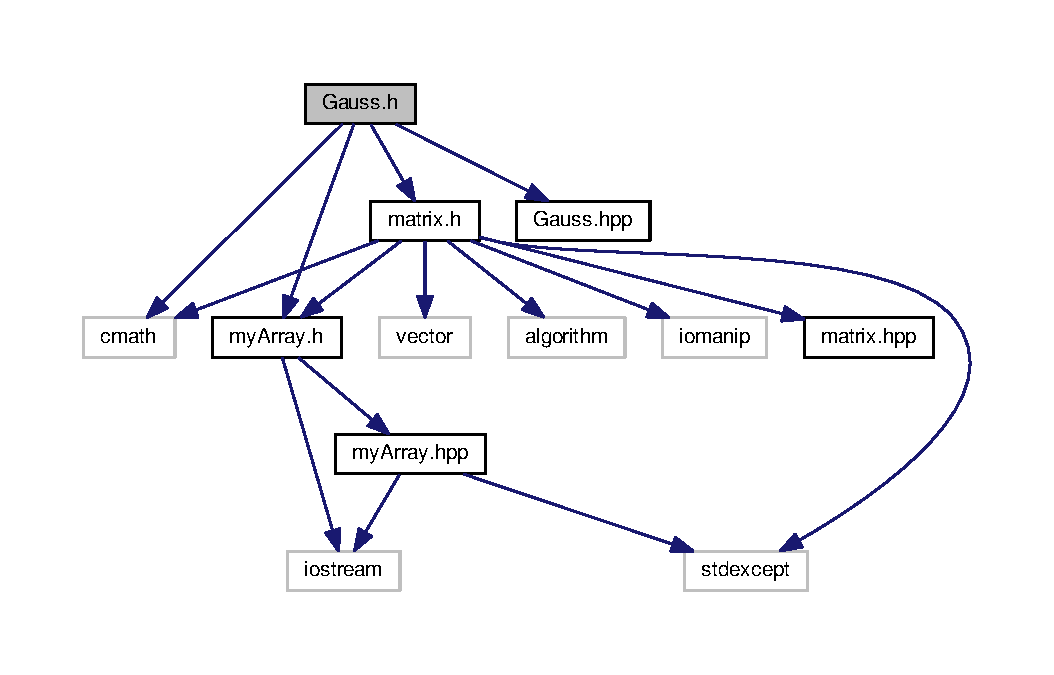
\includegraphics[width=350pt]{Gauss_8h__incl}
\end{center}
\end{figure}
\subsection*{Classes}
\begin{DoxyCompactItemize}
\item 
class \hyperlink{classGauss}{Gauss$<$ T $>$}
\end{DoxyCompactItemize}


\subsection{Detailed Description}
the \hyperlink{classGauss}{Gauss} class 
\hypertarget{matrix_8h}{}\section{matrix.\+h File Reference}
\label{matrix_8h}\index{matrix.\+h@{matrix.\+h}}
{\ttfamily \#include \char`\"{}my\+Array.\+h\char`\"{}}\\*
{\ttfamily \#include $<$vector$>$}\\*
{\ttfamily \#include $<$algorithm$>$}\\*
{\ttfamily \#include $<$cmath$>$}\\*
{\ttfamily \#include $<$iomanip$>$}\\*
{\ttfamily \#include $<$stdexcept$>$}\\*
{\ttfamily \#include \char`\"{}matrix.\+hpp\char`\"{}}\\*
Include dependency graph for matrix.\+h\+:\nopagebreak
\begin{figure}[H]
\begin{center}
\leavevmode
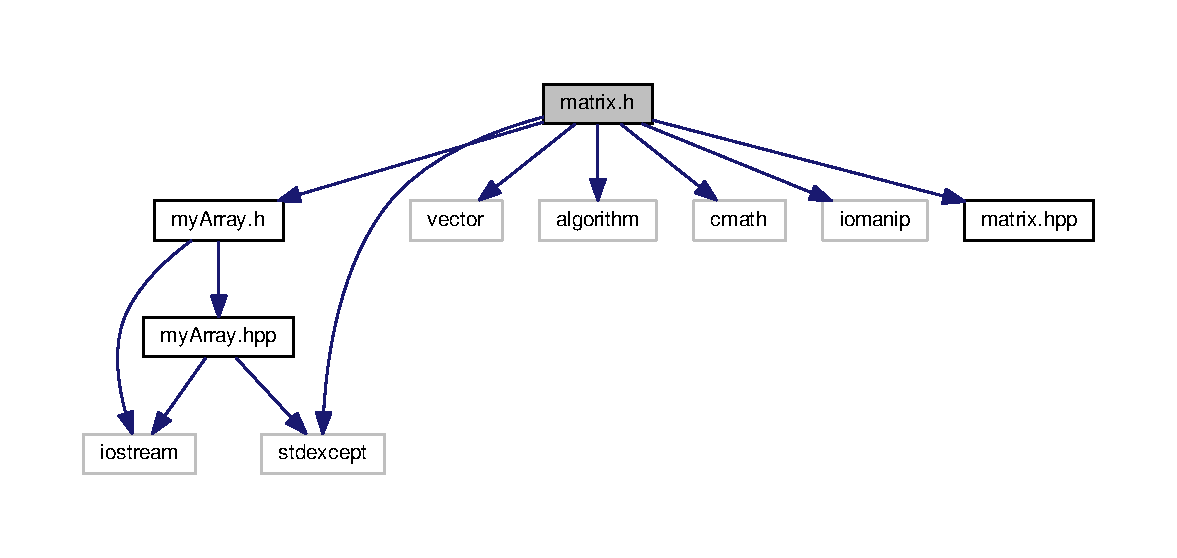
\includegraphics[width=350pt]{matrix_8h__incl}
\end{center}
\end{figure}
This graph shows which files directly or indirectly include this file\+:\nopagebreak
\begin{figure}[H]
\begin{center}
\leavevmode
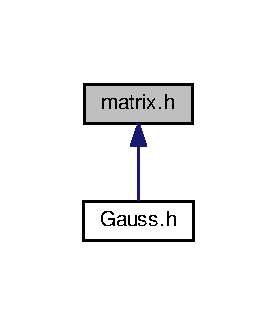
\includegraphics[width=133pt]{matrix_8h__dep__incl}
\end{center}
\end{figure}
\subsection*{Classes}
\begin{DoxyCompactItemize}
\item 
class \hyperlink{classMatrix}{Matrix$<$ T $>$}
\item 
class \hyperlink{classMatrix}{Matrix$<$ T $>$}
\item 
class \hyperlink{classCompare}{Compare$<$ T $>$}
\end{DoxyCompactItemize}
\subsection*{Functions}
\begin{DoxyCompactItemize}
\item 
{\footnotesize template$<$class T $>$ }\\ostream \& \hyperlink{matrix_8h_aabfdf243bf6d7e452fcef8553c128096}{operator$<$$<$} (ostream \&out, \hyperlink{classMatrix}{Matrix}$<$ T $>$ \&mat)
\end{DoxyCompactItemize}


\subsection{Detailed Description}
A \hyperlink{classMatrix}{Matrix} class. 

\subsection{Function Documentation}
\index{matrix.\+h@{matrix.\+h}!operator$<$$<$@{operator$<$$<$}}
\index{operator$<$$<$@{operator$<$$<$}!matrix.\+h@{matrix.\+h}}
\subsubsection[{\texorpdfstring{operator$<$$<$(ostream \&out, Matrix$<$ T $>$ \&mat)}{operator<<(ostream &out, Matrix< T > &mat)}}]{\setlength{\rightskip}{0pt plus 5cm}template$<$class T $>$ ostream\& operator$<$$<$ (
\begin{DoxyParamCaption}
\item[{ostream \&}]{out, }
\item[{{\bf Matrix}$<$ T $>$ \&}]{mat}
\end{DoxyParamCaption}
)}\hypertarget{matrix_8h_aabfdf243bf6d7e452fcef8553c128096}{}\label{matrix_8h_aabfdf243bf6d7e452fcef8553c128096}
Stream insertion operator for {\ttfamily \hyperlink{classMatrix}{Matrix}}.

\begin{DoxyPrecond}{Precondition}
Stream insertion operator is defined for {\ttfamily T}. 
\end{DoxyPrecond}
\begin{DoxyPostcond}{Postcondition}
The contents of the m\+\_\+matrix are printed to the ouptut stream. Each array is printed on a new row. 
\end{DoxyPostcond}
\begin{DoxyReturn}{Returns}
the modified output stream. 
\end{DoxyReturn}

\hypertarget{myArray_8h}{}\section{my\+Array.\+h File Reference}
\label{myArray_8h}\index{my\+Array.\+h@{my\+Array.\+h}}
{\ttfamily \#include $<$iostream$>$}\\*
{\ttfamily \#include \char`\"{}my\+Array.\+hpp\char`\"{}}\\*
Include dependency graph for my\+Array.\+h\+:\nopagebreak
\begin{figure}[H]
\begin{center}
\leavevmode
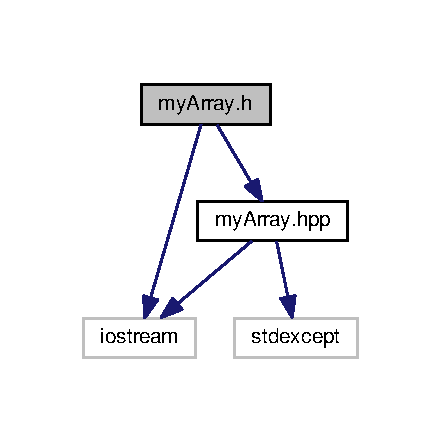
\includegraphics[width=212pt]{myArray_8h__incl}
\end{center}
\end{figure}
This graph shows which files directly or indirectly include this file\+:\nopagebreak
\begin{figure}[H]
\begin{center}
\leavevmode
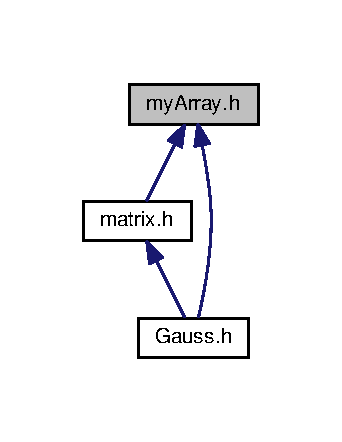
\includegraphics[width=164pt]{myArray_8h__dep__incl}
\end{center}
\end{figure}
\subsection*{Classes}
\begin{DoxyCompactItemize}
\item 
class \hyperlink{classMyArray}{My\+Array$<$ T $>$}
\item 
class \hyperlink{classMyArray}{My\+Array$<$ T $>$}
\end{DoxyCompactItemize}
\subsection*{Functions}
\begin{DoxyCompactItemize}
\item 
{\footnotesize template$<$class T $>$ }\\ostream \& \hyperlink{myArray_8h_af7b7cf0da2b1c59cd870d8d98066f286}{operator$<$$<$} (ostream \&out, \hyperlink{classMyArray}{My\+Array}$<$ T $>$ \&arr)
\end{DoxyCompactItemize}


\subsection{Detailed Description}
An Array class. 

\subsection{Function Documentation}
\index{my\+Array.\+h@{my\+Array.\+h}!operator$<$$<$@{operator$<$$<$}}
\index{operator$<$$<$@{operator$<$$<$}!my\+Array.\+h@{my\+Array.\+h}}
\subsubsection[{\texorpdfstring{operator$<$$<$(ostream \&out, My\+Array$<$ T $>$ \&arr)}{operator<<(ostream &out, MyArray< T > &arr)}}]{\setlength{\rightskip}{0pt plus 5cm}template$<$class T $>$ ostream\& operator$<$$<$ (
\begin{DoxyParamCaption}
\item[{ostream \&}]{out, }
\item[{{\bf My\+Array}$<$ T $>$ \&}]{arr}
\end{DoxyParamCaption}
)}\hypertarget{myArray_8h_af7b7cf0da2b1c59cd870d8d98066f286}{}\label{myArray_8h_af7b7cf0da2b1c59cd870d8d98066f286}
Stream insertion operator for {\ttfamily my\+Array}.

\begin{DoxyPrecond}{Precondition}
Stream insertion operator is defined for {\ttfamily T}. 
\end{DoxyPrecond}
\begin{DoxyPostcond}{Postcondition}
The contents of the interval\+Data are printed to the ouptut stream. 
\end{DoxyPostcond}
\begin{DoxyReturn}{Returns}
the modified output stream. 
\end{DoxyReturn}

%--- End generated contents ---

% Index
\backmatter
\newpage
\phantomsection
\clearemptydoublepage
\addcontentsline{toc}{chapter}{Index}
\printindex

\end{document}
